
%(BEGIN_QUESTION)
% Copyright 2011, Tony R. Kuphaldt, released under the Creative Commons Attribution License (v 1.0)
% This means you may do almost anything with this work of mine, so long as you give me proper credit

This override control system protects the diesel engine/generator from overheating under conditions where there is a high demand for electrical power in the grid:

$$\includegraphics[width=15.5cm]{i03790x01.eps}$$

Complete the following table of signal values for this system, assuming a high-load condition where the voltage controller (EIC) is being overridden by the temperature controller (TIC).  Note that there are ranges of correct answers here -- all I'm looking for is a set of values that would be realistic:

% No blank lines allowed between lines of an \halign structure!
% I use comments (%) instead, so that TeX doesn't choke.

$$\vbox{\offinterlineskip
\halign{\strut
\vrule \quad\hfil # \ \hfil & 
\vrule \quad\hfil # \ \hfil & 
\vrule \quad\hfil # \ \hfil \vrule \cr
\noalign{\hrule}
%
% First row
{\bf Parameter} & {\bf TIC-41} & {\bf EIC-35} \cr
%
\noalign{\hrule}
%
% Another row
PV &  &  \cr
%
\noalign{\hrule}
%
% Another row
SP & 220 deg F & 13,800 volts \cr
%
\noalign{\hrule}
%
% Another row
Output &  &  \cr
%
\noalign{\hrule}
} % End of \halign 
}$$ % End of \vbox

\underbar{file i03790}
%(END_QUESTION)





%(BEGIN_ANSWER)

{\it 3 points for TIC PV being equal or more than 220 deg F; 3 points for EIC PV being less than 13,800 volts; 4 points for EIC output being greater than TIC output.}

% No blank lines allowed between lines of an \halign structure!
% I use comments (%) instead, so that TeX doesn't choke.

$$\vbox{\offinterlineskip
\halign{\strut
\vrule \quad\hfil # \ \hfil & 
\vrule \quad\hfil # \ \hfil & 
\vrule \quad\hfil # \ \hfil \vrule \cr
\noalign{\hrule}
%
% First row
{\bf Parameter} & {\bf TIC} & {\bf EIC} \cr
%
\noalign{\hrule}
%
% Another row
PV & $\geq$ 220 deg F & $<$ 13,800 volts  \cr
%
\noalign{\hrule}
%
% Another row
SP & 220 deg F & 13,800 volts \cr
%
\noalign{\hrule}
%
% Another row
Output & $<$ EIC output & $>$ TIC output \cr
%
\noalign{\hrule}
} % End of \halign 
}$$ % End of \vbox

{\it Deduct 2 points for any answer that is absurd.  For example, saying the engine temperature is 1000 degrees F, or that the line voltage is 0 volts.}

%(END_ANSWER)





%(BEGIN_NOTES)

{\bf This question is intended for exams only and not worksheets!}.

%(END_NOTES)


